\documentclass[11pt]{article}
\usepackage{amsmath, amsthm, amssymb, pdfpages} 
\usepackage{fullpage}
\usepackage{hyperref}
\usepackage{graphicx}
\usepackage[capitalize]{cleveref}

% next three for UTF8 to work (for non-ASCII names to work without awkward codes)
\usepackage[T1]{fontenc}
\usepackage{textcomp}
\usepackage[utf8]{inputenc}

% import biblatex with prefered settings
% reuse code and library from LIGERA paper in the same repository
% loads biblatex with all the nice standard options that John determined some time ago!
% this version uses a ``Harvard'' style (first author last name, year in parentheses).
% also loads xpatch

% biblatex
% harvard style
\usepackage[style=authoryear,natbib,maxcitenames=2,doi=true,isbn=false,url=false,backend=bibtex]{biblatex}
% numeric style
%% \usepackage[style=numeric-comp,sorting=none,giveninits=true,
%%                      doi=false,isbn=false,url=false,backend=bibtex]{biblatex}
% remove "In: " before journal title
\renewbibmacro{in:}{}
% remove language
\AtEveryBibitem{\clearlist{language}}
% remove month
\AtEveryBibitem{\clearfield{month}}
% and also notes
\AtEveryBibitem{\clearfield{note}}
% remove dots between volume and issue
\usepackage{xpatch}
\xpatchbibmacro{volume+number+eid}{%
  \setunit*{\adddot}%
}{%
}{}{}
% put issue in parentheses
\DeclareFieldFormat[article]{number}{\mkbibparens{#1}}


\bibliography{zotero, dummy} % biblatex wants this in the preamble...

% copied from PCA-GWAS paper
\newcommand{\auc}{\text{AUC}_\text{PR}}

\usepackage[noT]{kinshipsymbols}
% % copy of \Fst from package `kinshipsymbols`

% some more definitions
\newcommand{\kinMat}{%
  \ensuremath{%
    \mathbf{\Phi}
  }%
  \xspace%
}%
\newcommand{\kinMatStdLim}{%
  \ensuremath{%
    \mathbf{\hat{\Phi}}^\text{std-lim}
  }%
  \xspace%
}%

% % for theorems!
% \usepackage{amsthm}
% %\newtheorem{thm}{Theorem}[section]
% \newtheorem*{thm}{Theorem}
% %\newtheorem{lem}[thm]{Lemma}
% \newtheorem*{lem}{Lemma}
% % \newtheorem{lemma}[theorem]{Lemma}

% % double line spacing (PLoS wants this)
% \usepackage{setspace}
% \doublespacing
% spacing smaller than double
\renewcommand{\baselinestretch}{1.2}

\title{\Large \textbf{The effect of population kinship estimation bias in structured genetic association studies}}
\author{Zhuoran Hou$^1$, Alejandro Ochoa$^{1,2,*}$}
\date{}

\begin{document}
\maketitle

\noindent
$^1$ Department of Biostatistics and Bioinformatics, Duke University, Durham, NC 27705, USA \\
$^2$ Duke Center for Statistical Genetics and Genomics, Duke University, Durham, NC 27705, USA \\
$^*$ Corresponding author: \texttt{alejandro.ochoa@duke.edu}


\begin{abstract}
  Population kinship matrices are estimated for a variety of applications, including control for population structure in genetic association studies.
  Recent work found that the most common kinship estimators can be severely biased.
  In this work, we investigate the effect of this kinship bias on the downstream application of genetic association.
  Remarkably, kinship bias does not affect genetic associations based on either Principal Components Analysis (PCA) or Linear Mixed-effects Models (LMM).
  We present empirical observations using simulated data, then prove association equivalence for specific biases theoretically using linear algebra.
  In particular, the exact form of the kinship bias is compensated for by fitting the intercept in both PCA and LMM approaches, which model population structure via covariates, suggesting that only models with this precise arrangement will be robust to this kinship bias.
\end{abstract}

\clearpage

\tableofcontents

\clearpage
	
\section{TO DO}

Plan for finishing paper.
Will pursue these items in this order:

\begin{itemize}
\item Prove WG equivalence just like for the standard kinship estimator.
  NOTE: I couldn't come up with a transformation like the centering matrix that carries over easily to the matrix square root, so it may be challenging.
\item Add a real genotype illustration (1000 Genomes).
  \begin{itemize}
  \item Adds smaller kinship matrix fig and p-value correlation fig.
  \end{itemize}
\end{itemize}


\clearpage

\section{Introduction}

% direct copy from Part II
Kinship is utilized in principal components analyses and linear-mixed effects models to correct for structure in Genome-Wide Association Studies (GWAS) \citep{xie_combining_1998,yu_unified_2006, aulchenko_genomewide_2007, price_principal_2006, astle_population_2009,kang_efficient_2008, kang_variance_2010, yang_gcta:_2011, zhou_genome-wide_2012, loh_efficient_2015, sul_population_2018}.
The most commonly-used kinship estimator \citep{price_principal_2006, astle_population_2009, rakovski_kinship-based_2009, thornton_roadtrips:_2010, yang_common_2010, yang_gcta:_2011, zhou_genome-wide_2012, speed_improved_2012, speed_relatedness_2015, loh_efficient_2015, wang_efficient_2017, sul_population_2018} was recently determined to have a complex bias \citep{weir_unified_2017, ochoa_estimating_2021}.

WG has a simpler, uniform bias \citep{weir_unified_2017, ochoa_estimating_2021}.

popkin is unbiased  \citep{ochoa_estimating_2021}.

\section{Results}

\subsection{Empirical demonstration of robustness to kinship bias in PCA and LMM genetic assocation studies}

To quantify the effect of the various kinship matrix estimators, and their limiting biases, we simulated genotypes and a trait, and calculated association p-values for all kinship variants of the PCA and LMM methods.
We first simulated an admixed population with $K=3$ ancestries, then simulated a 20-generation random pedigree from the admixed population as founders.
This high-dimensinal admixed family scenario results in a large difference in performance between PCA and LMM approaches \citep{yao_testing_2019}.
To further differentiate methods, we increase noise in kinship estimation by purposefully simulated a small number of loci, $m=10,000$.

% path for figures
\graphicspath{ {../data/sim-admix-n1000-m10000-k3-f0.3-s0.5-mc100-h0.8-g20-fes/} }

\begin{figure}[bp!]
  \centering
  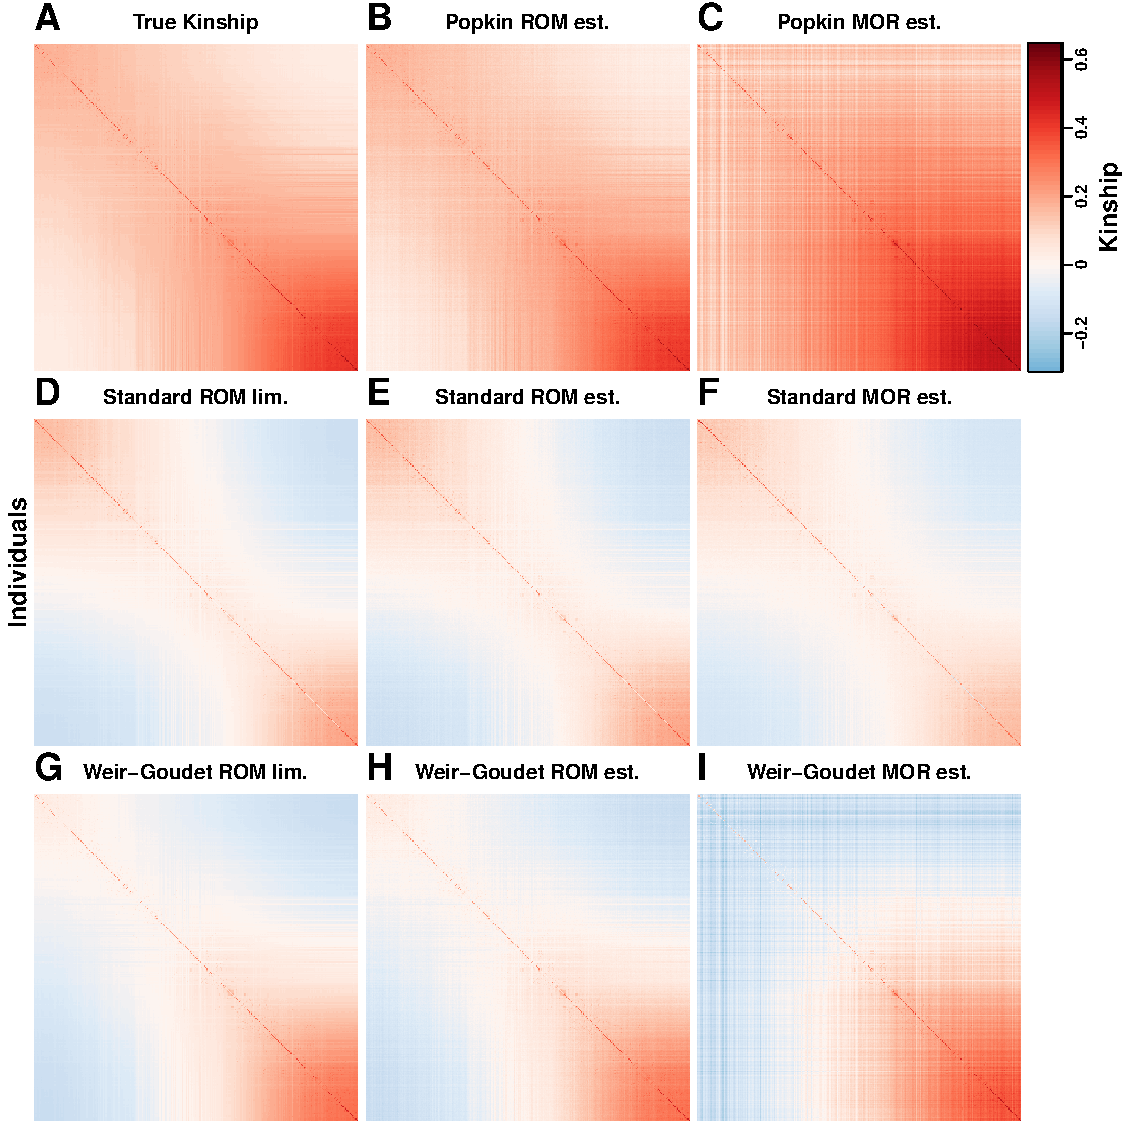
\includegraphics[height=0.8\textheight]{kinship.pdf}
  \caption{
    {\bf Kinship estimates and their limits on the admixed family simulation.}
    Each panel represents a kinship matrix as a heatmap, with each of the $n=1000$ individuals along both x and y axes, and the kinship value presented as color: positive estimates are in red, negative estimates in blue.
    The estimators considered are Popkin, Standard, GCTA, and Weir-Goudet.
    Each estimator has its limit in the first column (the limit of Popkin is Truth).
    Standard has two variants: ROM (ratio of means) and MOR (mean of ratios).
    Standard MOR does not have a closed-form limit, but in practice matches that of Standard ROM.
  }
  \label{fig:kinship}
\end{figure}

The kinship estimates on this simulation, and the theoretical limits of these estimators, are shown in \cref{fig:kinship}.
The true kinship matrix (\cref{fig:kinship}A) shows the family relatedness as high values concentrated near the diagonal and the ancestry-driven population structure as the broad patterns off-diagonal.
This simulation illustrates the severity of the biases of these estimators, which were previously characterized theoretically \citep{ochoa_estimating_2021}.
Only the Popkin estimator is unbiased (\cref{fig:kinship}B), the rest presenting large negative biases which in turn result in abundant negative estimates.
The Standard kinship estimator (the mean-of-ratios, or MOR, version; \cref{fig:kinship}E), which is the most common estimator in these applications, and the closely related ratio-of-means (ROM) estimator (\cref{fig:kinship}D), both have severe biases that are not only overall downwardly biased, but these biases also vary for every pair of individuals.
The limit of the Standard ROM estimator (\cref{fig:kinship}C), calculated from the true kinship matrix and its known functional form (see Methods), closely matches the previously mentioned estimates obtained from genotypes.
The GCTA estimator equals the Standard MOR estimator except for the diagonal values, which also have a different bias (\cref{fig:kinship}F-G).
Lastly, the Weir-Goudet estimator has a uniform downward bias (\cref{fig:kinship}H-I).

\begin{figure}[bp!]
  \centering
  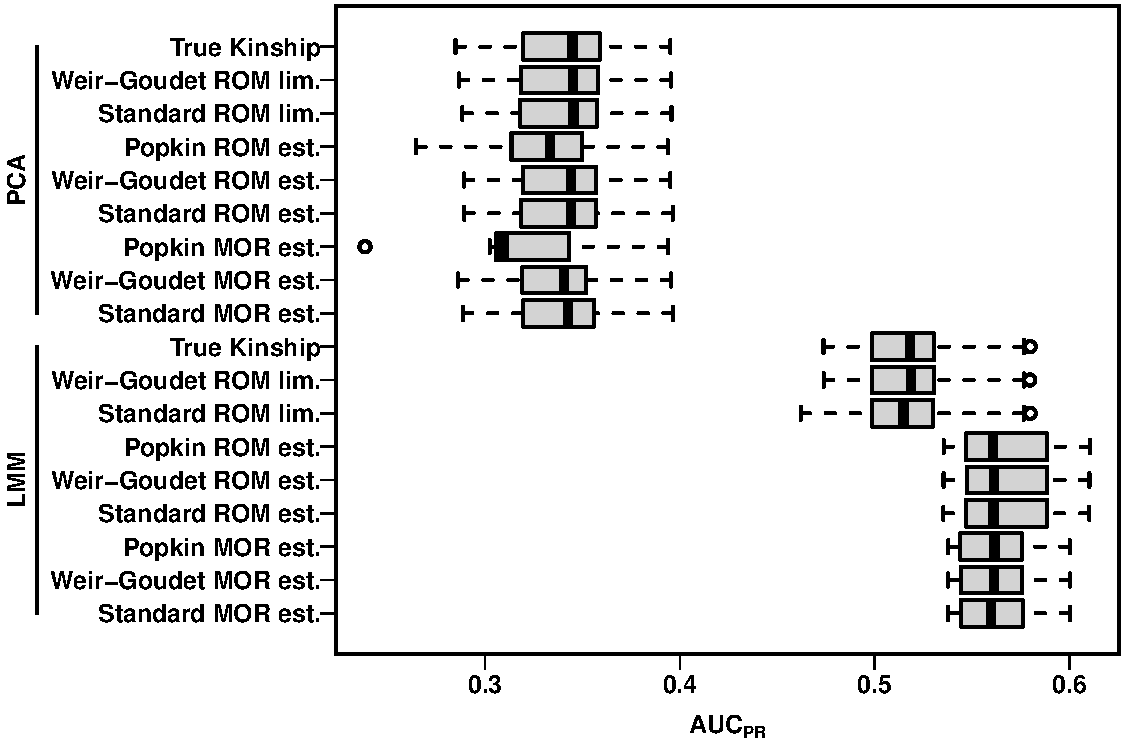
\includegraphics[width=\textwidth]{auc.pdf}
  \caption{
    {\bf Area Under the Precision-Recall Curves ($\auc$) for every combination of association model and kinship estimate.}
    Results based on a single replicate of the random genotype matrix and trait vector.
    Approaches appear to cluster primarily by association model (LMM vs PCA) and whether a kinship estimate was used or not, and do not depend much at all on the form of the bias.
  }
  \label{fig:auc}
\end{figure}

We then performed both LMM and PCA association tests in order to determine if the kinship biases carry over to association biases.
Surprisingly, we found that none of these kinship biases have discernible effects on association performance, as summarized by the Area Under the Precision-Recall Curve ($\auc$; \cref{fig:auc}).
The largest difference in performance is explained by the association model used (LMM vs PCA), as expected due to our use of a family simulation, where PCA is expected to perform less well than LMM.
For PCA only, there are no clear differences between the performance of any of the kinship matrices.
In contrast, the LMM results are relatively more sensitive to the use of noisy kinship estimates versus the (noiseless) limits of these estimates, a difference certainly increased by our deliberate use of a small number of simulated loci.
Among the kinship estimator limits, use of the true kinship matrix, the limit of the Weir-Goudet estimator, or the limit of the Standard ROM estimator all result in practically the same performance, while the limit of the GCTA estimator shows a difference in performance.
Similarly, among the estimates, the popkin, Weir-Goudet, and Standard ROM estimates result in the same performance, whereas the Standard MOR and GCTA estimates (which equals Standard MOR off-diagonal) have a slightly different performance.

\begin{figure}[bp!]
  \centering
  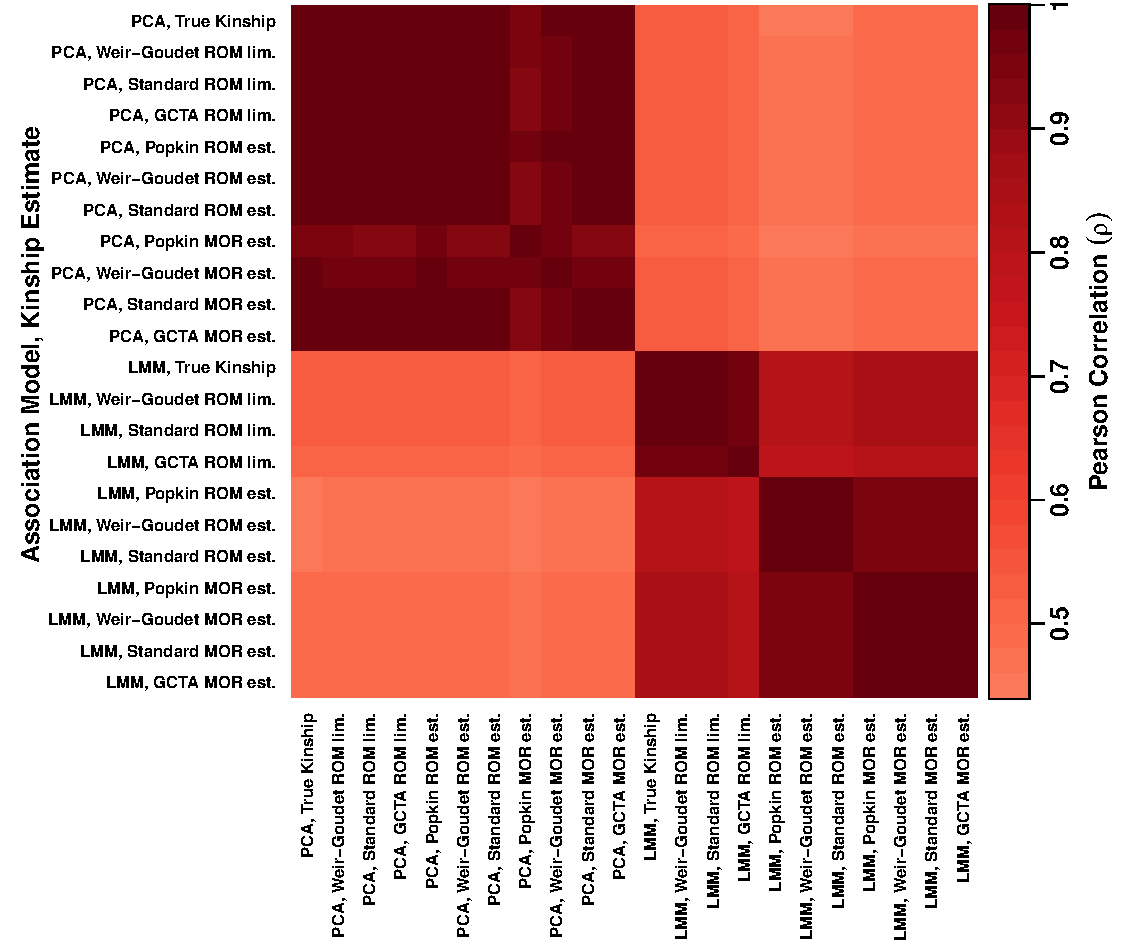
\includegraphics[width=\textwidth]{pvals_cor.pdf}
  \caption{
    {\bf Correlation between p-values of different association models and kinship estimates.}
    The association p-value vector (one value per tested locus) produced by each combination of association model (LMM vs PCA) and kinship matrix (x and y axes) was used to compute Pearson correlations (color).
    P-values between all kinship matrices using the same association model (PCA or LMM) are highly correlated (including biased and unbiased estimates), and often the maximum correlation of 1 is achieved.
  }
  \label{fig:pvals_cor}
\end{figure}

To better understand the degree of agreement between the association results of the various kinship matrices, we next measured the agreement between methods at the level of the individual association p-values, summarized using pearson correlation coefficients ($\rho$; \cref{fig:pvals_cor}).
We found that all the kinship matrices yield highly correlated p-values when applied to the same association model (LMM vs PCA), and otherwise mirroring our previous observations based on $\auc$.
The minimum correlation among PCA methods was $0.86$, and among LMMs it was $0.84$.
Within PCA, the cluster that excludes the true kinship matrix and the popkin estimate has nearly identical p-values ($\rho > 0.99$), and inclusion of popkin lowers the minimum correlation to $\rho > 0.93$.
Among LMMs, the cluster that includes the true kinship and the Weir-Goudet and Standard ROM limits also results in practically identical p-values ($\rho \approx 1$), while including the GCTA limit lowers that to $\rho > 0.97$.
The LMM cluster that includes the Popkin, Weir-Goudet, and Standard ROM estimators also has $\rho \approx 1$, and separately the cluster with the Standard MOR and GCTA estimators has $\rho \approx 1$, while the LMM cluster that includes all estimates has $\rho > 0.96$.
Thus, several sets of kinship matrices with different biases result in identical association statistics, within both LMMs and PCA models, while differences are largely driven by the association model used and whether the kinship matrices were estimates or not.

% \begin{figure}[bp!]
%   \centering
%   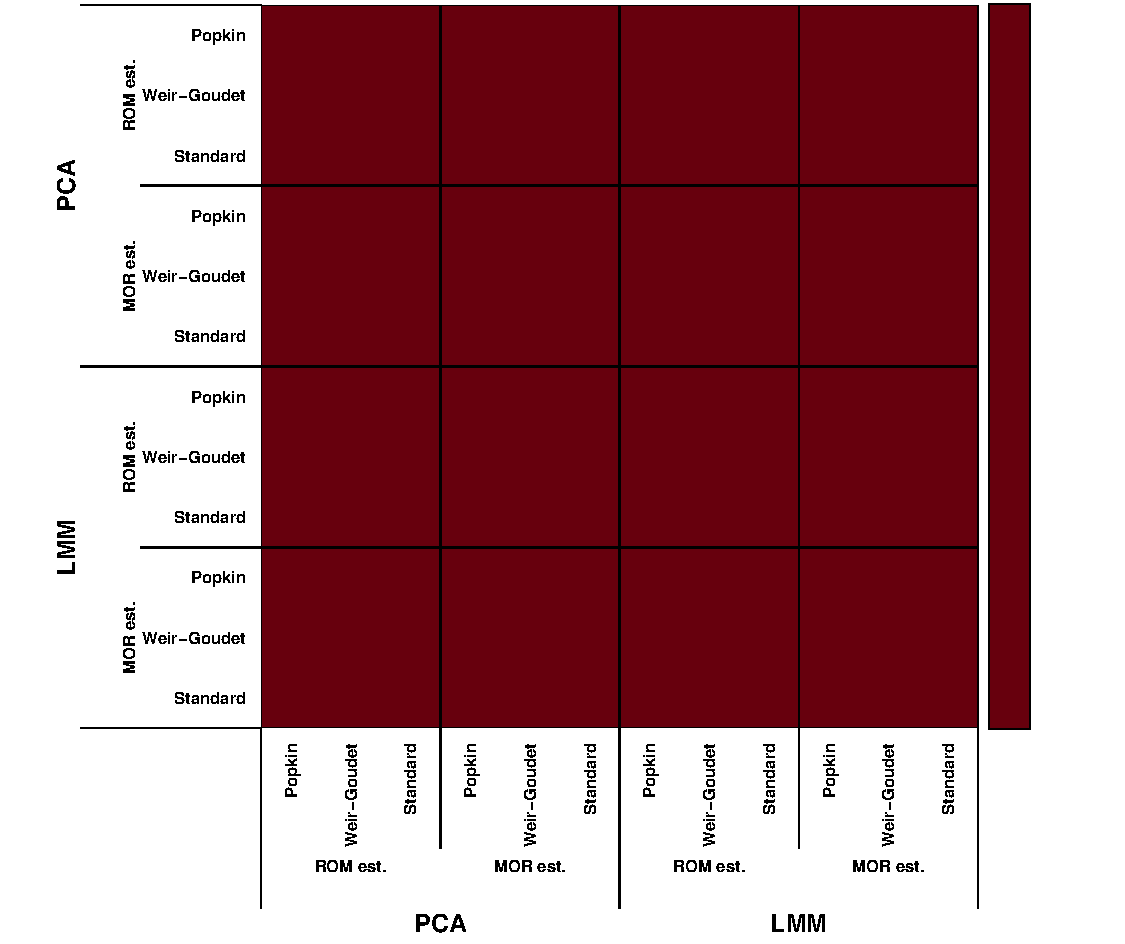
\includegraphics[width=3in]{betas_cor.pdf}
%   \caption{
%     {\bf Heatmap and dendrogram for $\hat{\mathbf{\beta}}$ of GCTA and PCA with different kinship matrices ($m=10,000$).}
%   }
%   \label{fig:betas_cor}
% \end{figure}

\subsection{Theoretical justification of empirical observations under standard kinship bias}

Our empirical observations suggested that the biases of the Standard kinship estimator do not alter association statistics whatsoever; here we provide proof that this is indeed the case.
To eliminate random estimation noise from the analysis (which our empirical evaluations suggest play a minor role), we shall focus exclusively on the limiting bias of the Standard (ROM) kinship estimator.
Our constructive proof identifies the exact conditions that allows the kinship bias to be compensated for, namely that population structure is modeled as a (fixed or random effect) covariate and an intercept term is fit jointly.
More specifically, we find that the coefficients of the intercept and the random effect or PCs (for LMM and PCA, respectively) adapt to the bias, and no other coefficients change.
This is fortunate, as the intercept and random effects or PCs coefficients are nuisance parameters that are most often unreported, while the focal genetic association coefficient and its p-value are completely unchanged by this precise bias.

Our theoretical results only consider the true kinship matrix \kinMat and the limit of the standard kinship estimator (see \textbf{Methods}, \cref{eq:kinship_std_lim}), which can be stated in matrix notation as
$$
\kinMatStdLim
=
\frac{1}{1 - \bar{\varphi}}
\left(
  \kinMat
  + \bar{\varphi} \mathbf{J}
  - \boldsymbol{\varphi} \mathbf{1}^\intercal 
  - \mathbf{1} \boldsymbol{\varphi}^\intercal 
\right)
,
$$
where
$\mathbf{1}$ is a length-$n$ column vector of ones,
$\mathbf{J} = \mathbf{1} \mathbf{1}^\intercal$ is the $n \times n$ matrix full of ones,
$\boldsymbol{\varphi} = \frac{1}{n} \mathbf{1}^\intercal \kinMat$ is a length-$n$ vector of per-row mean kinship values, and
$\bar{\varphi} = \frac{1}{n^2} \mathbf{1}^\intercal \kinMat \mathbf{1}$ is the overall mean kinship (scalar).
The two kinship matrices are related more succinctly using the $n \times n$ centering matrix,
$$
\mathbf{C}
=
\mathbf{I} - \frac{1}{n} \mathbf{J},
$$
where $\mathbf{I}$ is the $n \times n$ identity matrix.
The limit of the standard kinship estimator is given in terms of a transformation of the true kinship matrix by
\begin{equation}
  \label{eq:kin-std-lim-C}
  \kinMatStdLim
  =
  \frac{1}{1 - \bar{\varphi}}
  \mathbf{C} \kinMat \mathbf{C}
  .
\end{equation}

The centering matrix has been well studied, and we review its properties here.
For any length-$n$ vector $\mathbf{v}$ we have
\begin{align*}
  \mathbf{C} \mathbf{v}
  % =
  % \left(\mathbf{I} - \frac{1}{n} \mathbf{1} \mathbf{1}^\intercal\right) \mathbf{v}
  % =
  % \mathbf{I} \mathbf{v} - \frac{1}{n} \mathbf{1} \mathbf{1}^\intercal \mathbf{v}
  =
  \mathbf{v} - \mathbf{1} \bar{v}
  ,
\end{align*}
where $\bar{v} = \frac{1}{n} \mathbf{1}^\intercal \mathbf{v}$ is the mean value of the elements of $\mathbf{v}$.
Therefore, $\mathbf{v} = \mathbf{1}$ gets transformed to the zero vector, so it is an eigenvector with an eigenvalue of zero:
\begin{align*}
  \mathbf{C} \mathbf{1}
  % =
  % \mathbf{1} - \mathbf{1}
  =
  \mathbf{0}
  .
\end{align*}
Moreover, any vector $\mathbf{v}$ orthogonal to $\mathbf{1}$ has a zero mean element ($\bar{v} = 0$) by hypothesis and it is not altered by $\mathbf{C}$ ($\mathbf{C} \mathbf{v} = \mathbf{v}$).
Therefore, the nullspace of $\mathbf{C}$ is spanned by $\mathbf{1}$.

This centering matrix provides the key insight as to why LMM and PCA approaches are robust to this specific kinship bias, namely that the bias in the random effects (for LMM) or eigenvectors (for PCA) of \kinMatStdLim results in removing the mean values of these covariates only, so fitting the intercept term $\mathbf{1} \alpha$ compensates exactly for this bias.
In the remaining sections we detail this argument, where we construct equivalent solutions under the true and biased kinship matrices.

% First we show the following lemma.

% \begin{lem}
%   $\mathbf{1}$ is in the nullspace of \kinMatStdLim but not of \kinMat.
% \end{lem}

% \begin{proof}
% The vector $\mathbf{1}$ is not in the nullspace of any true kinship matrix \kinMat, since $\kinMat \mathbf{1} \neq \mathbf{0}$, which follows since all kinship values are non-negative and the diagonal of the kinship matrix is strictly positive (it has a minimum value of $\frac{1}{2}$).
% However, $\mathbf{1}$ is in the nullspace of \kinMatStdLim since $\mathbf{C} \mathbf{1} = \mathbf{0}$:
% $$
% \kinMatStdLim \mathbf{1}
% =
% \frac{1}{1 - \bar{\varphi}}
% \mathbf{C} \kinMat \mathbf{C} \mathbf{1}
% =
% \mathbf{0}
% .
% $$
% \end{proof}

% Now we may prove the desired theorem.

% \begin{thm}
%   The rowspace of \kinMat and $\mathbf{1}$ equals rowspace of \kinMatStdLim and $\mathbf{1}$.
% \end{thm}

% \begin{proof}
%   Since $\mathbf{1}$ is in both rowspaces, it suffices to consider vectors $\mathbf{v}$ orthogonal to $\mathbf{1}$, which satisfy $\mathbf{C} \mathbf{v} = \mathbf{v}$.
%   We shall prove below that any such vector is in the nullspace of \kinMat if and only if it is in the nullspace of \kinMatStdLim.
%   Then, since the nullspace of \kinMat and $\mathbf{1}$ is the same as the nullspace of \kinMatStdLim and $\mathbf{1}$, it follows from the fundamental theorem of linear algebra that their rowspaces are also the same.
  
%   If $\mathbf{v}$ is in the nullspace of \kinMat, then $\kinMat \mathbf{v} = \mathbf{0}$.
%   It follows that
%   $$
%   \kinMatStdLim \mathbf{v}
%   =
%   \frac{1}{1 - \bar{\varphi}}
%   \mathbf{C} \kinMat \mathbf{C} \mathbf{v}
%   =
%   \frac{1}{1 - \bar{\varphi}}
%   \mathbf{C} \kinMat \mathbf{v}
%   =
%   \mathbf{0}
%   ,
%   $$
%   so $\mathbf{v}$ is also in the nullspace of \kinMatStdLim.
  
%   Conversely, if $\mathbf{v}$ is in the nullspace of \kinMatStdLim, then $\kinMatStdLim \mathbf{v} = \mathbf{0}$, which implies that
%   $
%   \mathbf{C} \kinMat \mathbf{C} \mathbf{v}
%   =
%   \mathbf{C} \kinMat \mathbf{v}
%   =
%   \mathbf{0}
%   $.
%   Left multiplying by $\mathbf{v}^\intercal$ results in
%   $
%   \mathbf{v}^\intercal \mathbf{C} \kinMat \mathbf{v}
%   =
%   \mathbf{v}^\intercal \kinMat \mathbf{v}
%   =
%   0
%   $, which implies that $\mathbf{v}$ is also in the nullspace of the positive-semidefinite matrix \kinMat, as desired.
%   If \kinMat were positive definite, then no such $\mathbf{v} \ne \mathbf{0}$ would exist (\kinMat would have the trivial nullspace $\{ \mathbf{0} \}$).
% \end{proof}

\subsubsection{Kinship matrix square root}

% https://en.wikipedia.org/wiki/Square_root_of_a_matrix

Here we shall consider decompositions of positive semidefinite matrices of the form $\mathbf{\Sigma} = \mathbf{B} \mathbf{B}^\intercal$, which are guaranteed to exist.
We denote such a $\mathbf{B}$ as a square root of $\mathbf{\Sigma}$, or in short $\mathbf{B} = \mathbf{\Sigma}^\frac{1}{2}$.
These square roots of $\mathbf{\Sigma}$ are not unique, which is not a problem for our following argument; any such square root will work.
(Note that there are alternate definitions of matrix square roots, such as $\mathbf{\Sigma} = \mathbf{B} \mathbf{B}$, but due to its connection to covariance, the definition $\mathbf{\Sigma} = \mathbf{B} \mathbf{B}^\intercal$ we adopted is most natural for this work and the notation $\mathbf{B} = \mathbf{\Sigma}^\frac{1}{2}$ simplifies our arguments.)

Given a square root of the true kinship matrix, $\kinMat^\frac{1}{2}$, we can construct a square root of the limit of the standard kinship estimator as
\begin{equation}
  \label{eq:eq:kin-std-lim-C-sqrt}
  \left( \kinMatStdLim \right)^\frac{1}{2}
  =
  \frac{1}{ \sqrt{ 1 - \bar{\varphi} } }
  \mathbf{C} \kinMat^\frac{1}{2}
  .
\end{equation}
It can be directly verified that this matrix square root indeed satisfies
$\left( \kinMatStdLim \right)^\frac{1}{2} \left( \left( \kinMatStdLim \right)^\frac{1}{2} \right)^\intercal = \kinMatStdLim$
as given in \cref{eq:kin-std-lim-C}.

\subsubsection{The LMM genetic association model}

In genetic association we are given data for $n$ individuals, namely a length-$n$ vector of trait values $\mathbf{y}$, which correspond to a quantitative trait, and a length-$n$ vector $\mathbf{x}_i$ of genotypes at each locus $i$.
These genotypes are encoded as dosages for a given risk allele that varies for each locus $i$, so it takes on the values of 0, 1, or 2 for diploid individuals.
The goal is to determine if there is a significant association between the trait and the genotype vectors.
Most genetic association models are formulated as, or are equivalent to, regression models.

The LMM regression model is given by
\begin{equation}
  \label{eq:lmm_gwas}
  \mathbf{y}
  =
  \mathbf{1} \alpha + \mathbf{x}_i \beta + \mathbf{s} + \boldsymbol{\epsilon}
  ,
\end{equation}
where $\alpha$ is the intercept coefficient,
$\beta$ is the genetic effect coefficient,
$\boldsymbol{\epsilon}$ are random independent residuals ($\boldsymbol{\epsilon} \sim \text{Normal}(\mathbf{0}, \mathbf{I} \sigma^2_\epsilon)$ for some $\sigma^2_\epsilon$),
and the random effect satisfies \citep{sul_population_2018}
$$
\mathbf{s} \sim \text{Normal} \left( \mathbf{0}, \sigma^2 \kinMat \right),
$$
where $\sigma^2$ is also fit to the data.
The dependence of the model on \kinMat is clearer by writing it equivalently as
\begin{equation}
  \label{eq:lmm_gwas2}
  \mathbf{y}
  =
  \mathbf{1} \alpha + \mathbf{x}_i \beta + \sigma \kinMat^\frac{1}{2} \mathbf{r} + \boldsymbol{\epsilon}
  ,
\end{equation}
where $\mathbf{r} \sim \text{Normal} \left( \mathbf{0}, \mathbf{I} \right)$.
The equivalence of \cref{eq:lmm_gwas} and \cref{eq:lmm_gwas2} follows since $\mathbf{r}$ being Multivariate Normal implies that the affine transformation $\mathbf{s} = \sigma \kinMat^\frac{1}{2} \mathbf{r}$ is also Multivariate Normal, with matching mean and covariance of the desired $\mathbf{s}$, namely
\begin{align*}
  \E[ \mathbf{s} ]
  &=
    \sigma \kinMat^\frac{1}{2} \E[ \mathbf{r} ]
    = \mathbf{0},
  \\
  \Cov( \mathbf{s} )
  &= \left( \sigma \kinMat^\frac{1}{2} \right) \Cov( \mathbf{r} ) \left( \sigma \kinMat^\frac{1}{2} \right)^\intercal
    = \sigma^2 \kinMat
    .
\end{align*}
Note that the equivalence holds for every square root of \kinMat (all $\mathbf{s} = \sigma \kinMat^\frac{1}{2} \mathbf{r}$ are equal in distribution), since the only requirement for equivalence,
$\left( \kinMat^\frac{1}{2} \right) \left( \kinMat^\frac{1}{2} \right)^\intercal = \kinMat$,
is satisfied by hypothesis.

\subsubsection{Equivalent LMM fit under standard kinship bias}

In the LMM of \cref{eq:lmm_gwas2}, $\mathbf{y}$, $\mathbf{x}_i$, and \kinMat are given, while the coefficients $\alpha$, $\beta$, $\sigma$, and the random effects $\mathbf{r}$ and $\boldsymbol{\epsilon}$ are fit to this data.
This data is typically fit using maximum likelihood (ML) or restricted maximum likelihood (REML) \citep{kang_efficient_2008}; our argument covers any likelihood-based approach, since we will establish a parameter map between both models that results in equal likelihoods for every parameter set in the map.

We shall consider two model fits, one where \kinMat is given, while in the other we provide $\kinMat' = \kinMatStdLim$ instead.
The first fit will result in the unprimed variables below, while we distinguish the second fit using primed variables, namely:
\begin{align*}
  \mathbf{y}
  &=
    \mathbf{1} \alpha + \mathbf{x}_i \beta + \sigma \kinMat^\frac{1}{2} \mathbf{r} + \boldsymbol{\epsilon}
  \\
  &=
    \mathbf{1} \alpha' + \mathbf{x}_i \beta' + \sigma' \left( \kinMat' \right)^\frac{1}{2} \mathbf{r}' + \boldsymbol{\epsilon}'
    .
\end{align*}
Now we shall construct coefficients for the second model that result in the same fit to the data, including the same likelihood, as the first model.
We achieve this by first setting
$\beta' = \beta$,
$\boldsymbol{\epsilon}' = \boldsymbol{\epsilon}$,
and
$\mathbf{r}' = \mathbf{r}$.
Note that the previous equal random effects (including residuals) immediately results in the same likelihood for both models.
The only parameters left to construct are $\alpha'$ and $\sigma'$, which must satisfy
$$
\mathbf{1} \alpha  + \sigma \kinMat^\frac{1}{2} \mathbf{r}
=
\mathbf{1} \alpha' + \sigma' \left( \kinMat' \right)^\frac{1}{2} \mathbf{r}
.
$$
Next we substitute $\kinMat' = \kinMatStdLim$ using the matrix square root determined in terms of \kinMat in \cref{eq:eq:kin-std-lim-C-sqrt}, which results in
$$
\mathbf{1} \alpha  + \sigma \kinMat^\frac{1}{2} \mathbf{r}
=
\mathbf{1} \alpha' + \sigma'
\frac{1}{ \sqrt{ 1 - \bar{\varphi} } }
\mathbf{C} \kinMat^\frac{1}{2}
\mathbf{r}
.
$$
The unknowns are solved for by left-multiplying, in turns, by $\mathbf{C}$ (which makes terms with $\mathbf{1}$ vanish) and by $\mathbf{1}^\intercal$ (which makes the term with $\mathbf{C}$ vanish).
In the first case, left-multiplying by $\mathbf{C}$ results in
$$
\sigma \mathbf{C} \kinMat^\frac{1}{2} \mathbf{r}
=
\sigma'
\frac{1}{ \sqrt{ 1 - \bar{\varphi} } }
\mathbf{C} \kinMat^\frac{1}{2}
\mathbf{r}
,
$$
so the only value of the scalar $\sigma'$ that satisfies this equation is
$$
\sigma'
=
\sigma \sqrt{ 1 - \bar{\varphi} }
.
$$
In the second case, left-multiplying by $\mathbf{1}^\intercal$, while noting that $\mathbf{1}^\intercal \mathbf{1} = n$, and solving for $\alpha'$ results in
$$
\alpha'
=
\alpha  + \sigma \frac{1}{n} \mathbf{1}^\intercal \kinMat^\frac{1}{2} \mathbf{r}
.
$$

We just determined that every solution in terms of the true kinship matrix (including every combination of fixed coefficients and random effects) has a corresponding solution in terms of the limit of the standard kinship estimator, which has equal likelihood and equal fit to the data.
This includes the optimal solution, whether determined by the ML or REML criteria.
In both cases, the coefficient for the genetic effect is identical ($\beta' = \beta$ above), and because the fit to the data is also equal (in terms of likelihood and/or residuals), the association p-value is also equal (whether determined from the likelihood or from residuals).
Thus, while two coefficients (the intercept $\alpha$ and the random effect variance scale $\sigma^2$) vary depending on whether the true or the limit of the biased standard kinship estimator are used, these are both nuisance parameters as far as the association test is concerned.
The focal genetic effect coefficient and significance statistic are both invariant under this particular kinship bias compared to using the true kinship matrix.

\subsubsection{The PCA genetic association model}

The argument we just presented for LMM equivalence can be made with small changes for the PCA regression model, since these two models are so similar.
Here we shall state the PCA model and elaborate on its strong connection to the LMM model, which has been presented before in similar forms \citep{astle_population_2009, hoffman_correcting_2013}.

The PCA regression model is
\begin{equation}
  \label{eq:pca_gwas}
  \mathbf{y}
  =
  \mathbf{1} \alpha + \mathbf{x}_i \beta + \mathbf{U}_d \boldsymbol{\gamma}_d + \boldsymbol{\epsilon}
  ,
\end{equation}
where
$d$ is the number of principal components,
$\mathbf{U}_d$ is the $n \times d$ matrix of top eigenvectors (often refered to as ``principal components'' in genetics),
and $\boldsymbol{\gamma}_d$ is a length-$d$ vector of coefficients for each eigenvector.
Note that the only difference from the LMM model (\cref{eq:lmm_gwas2}) is the replacement of $\sigma \kinMat^\frac{1}{2} \mathbf{r}$ with $\mathbf{U}_d \boldsymbol{\gamma}_d$ here.

Before proceeding with our proof for invariance under the PCA model, to enhance our intuition of these two models, we present the relationship between eigendecomposition and matrix square roots, which helps us connect the PCA model firmly to the LMM.
Denote the eigendecomposition of the true kinship matrix as
$$
\kinMat = \mathbf{U} \mathbf{\Lambda} \mathbf{U}^\intercal,
$$
where $\mathbf{U}$ is the complete $n \times n$ matrix of eigenvectors, and
$\mathbf{\Lambda}$ is the $n \times n$ diagonal matrix of eigenvalues.
%The matrix of eigenvectors is orthogonal, so $\mathbf{U}^{-1} = \mathbf{U}^\intercal$.
Therefore, one square root of \kinMat is given by
$$
\kinMat^\frac{1}{2}
=
\mathbf{U} \mathbf{\Lambda}^\frac{1}{2}
,
$$
where $\mathbf{\Lambda}^\frac{1}{2}$ simply contains the square roots of each eigenvalue along the diagonal.
This equation reveals that the LMM model in \cref{eq:lmm_gwas2} can be written in terms of the eigendecomposition, and thus resemble the PCA model even more closely, since
$$
\sigma \kinMat^\frac{1}{2} \mathbf{r}
=
\sigma \mathbf{U} \mathbf{\Lambda}^\frac{1}{2} \mathbf{r}
=
\mathbf{U} \boldsymbol{\gamma}
,
$$
so that the length-$n$ vector $\boldsymbol{\gamma}$ of coefficients for all the $n$ eigenvectors is given by
$
\boldsymbol{\gamma} = \sigma \mathbf{\Lambda}^\frac{1}{2} \mathbf{r}
$.
Thus, the PCA model attempts to fit coefficients only for the top $d$ eigenvectors, whereas the LMM model effectively fits all of these coefficients by constraining them to a distribution.

\subsubsection{Approximately equivalent PCA fit under standard kinship bias}

We shall again consider two alternate model fits, here based on the PCA model of \cref{eq:pca_gwas}, one where the eigenvector matrix $\mathbf{U}_d$ corresponds to the true kinship matrix, and in the other $\mathbf{U}_d'$ corresponds to the biased limit of the standard kinship estimator.
They key approximation is that
$$
\mathbf{U}_d' \approx \mathbf{C} \mathbf{U}_d,
$$
which is not strictly equal (since $\mathbf{C} \mathbf{U}$ is not orthogonal, as eigenvectors must be), but we have found it to be a good approximation in practice.

The two model fits we are considering are
\begin{align*}
  \mathbf{y}
  &=
    \mathbf{1} \alpha + \mathbf{x}_i \beta + \mathbf{U}_d \boldsymbol{\gamma}_d + \boldsymbol{\epsilon}
  \\
  &=
    \mathbf{1} \alpha' + \mathbf{x}_i \beta' + \mathbf{U}_d' \boldsymbol{\gamma}_d' + \boldsymbol{\epsilon}'
    ,
\end{align*}
and we again assume that the focal parameter $\beta' = \beta$ and the residuals $\boldsymbol{\epsilon}' = \boldsymbol{\epsilon}$ are equal.
Eliminating the resulting shared terms, and replacing $\mathbf{U}_d' = \mathbf{C} \mathbf{U}_d$ (assuming that our approximation holds exactly) results in the remaining coefficients having to satisfy
$$
\mathbf{1} \alpha + \mathbf{U}_d \boldsymbol{\gamma}_d
=
\mathbf{1} \alpha' + \mathbf{C} \mathbf{U}_d \boldsymbol{\gamma}_d'.
$$
We solve for the missing coefficients by left-multiplying by $\mathbf{C}$ and $\mathbf{1}^\intercal$ as before, which here ultimately results in
\begin{align*}
  \boldsymbol{\gamma}_d'
  =
    \boldsymbol{\gamma}_d
  ,
  \quad\quad
  \alpha'
  =
    \alpha + \frac{1}{n} \mathbf{1}^\intercal \mathbf{U}_d \boldsymbol{\gamma}_d
    .
\end{align*}
Thus, as for LMM, here the nuisance intercept coefficient compensates for the bias in the eigenvectors.

The PCA regression is an ordinary multiple linear regression, which is fit by minimizing the sum of square residuals.
Since the residuals were equal in both models, then the optimal solution in one model maps to the optimal solution in the other model as well.
The p-value of the genetic effect is usually calculated using a chi-squared test or an F-test, both of which depend only on the residuals and the degrees of freedom, all of which are invariant under the solution parameter map we constructed.
Therefore, both the focal genetic effect coefficient $\beta$ and its p-value are invariant under this particular kinship bias compared to using the true kinship matrix.
However, the result for PCA relies on an approximation, whereas for LMM it was exact.

\subsection{Proof that WG is equivalent to true kinship in its random effects}

\subsubsection{The LMM genetic association model under Weir-Goudetkinship estimator}

Base on the equation below:

\[
\widehat{\Phi^{WG}}=\frac{1}{1-\tilde{\varphi}}(\boldsymbol{\Phi}-\tilde{\varphi}\boldsymbol{\mathrm{J}})W
\]

We could also express $\widehat{\Phi^{WG}}$ in this way:

\[
\varPhi=p\widehat{\Phi^{WG}}+q\mathrm{\mathbf{J}},
\]

where p and q are coefficients that adjust the bias between Weir-Goudet
kinship estimator and the true estimator. Specifically,

\[
p=1-\tilde{\varphi},q=\tilde{\varphi}.
\]

We denote the random effect the LMM using Weir-Goudet kinship estimator
$s^{WG}$, thus it satisfies:

\[
s^{WG}\sim N(\mathbf{0},\widehat{\Phi^{WG}}).
\]

In the LMM using true kinship matrix $\Phi$, we denote the random
effect s, which satisfies:

\[
s\sim N(\mathbf{0},\frac{1}{p}\mathbf{\varPhi})
\]

From the equation above, we could assume:

\[
s=s^{WG}+\eta\mathbf{1},
\]

where:

\[
\eta\sim N(\mathbf{0},\sigma_{\eta}^{2}),\eta\mathbf{1}\sim N(\mathbf{0},\sigma_{\eta}^{2}\mathbf{J})
\]

and $\eta\mathbf{1}$ should be independent to $s^{WG}$.

This matches the mean of covariance of the desired s, namely

\[
E(s)=\mathbf{0}
\]

\[
Cov(s)=Cov(s^{WG})+Cov(\eta\mathbf{1})=\frac{1}{p}\mathbf{\Phi}.
\]

From this equation, we could know that $\sigma_{\eta}^{2}=\frac{\tilde{\varphi}}{1-\tilde{\varphi}}.$

\subsubsection{Equivalent LMM fit under Weir-Goudet kinship bias}

Similarly, we consider two LMM fit: one we use s based on true kinship
matrix $\mathbf{\Phi}$, while in the other we use $s^{WG}$ which
based on Weir-Goudet kinship estimator:

\[
y=\alpha\mathbf{1}+\beta\mathbf{X}+\gamma s+\epsilon=\alpha^{'}\mathbf{1}+\beta^{'}\mathbf{X}+\gamma^{'}s^{WG}+\epsilon^{'}.
\]

Now, we want to construct coefficients in the second model that results
in the same fit as the first model using the truth kinship matrix.
We could first set $\beta=\beta^{'},\epsilon=\epsilon'$. As a results,
we only need to construct $\alpha'$ and $\gamma'$, which must satisfy:

\[
\alpha\mathbf{1}+\gamma s=\alpha^{'}\mathbf{1}+\gamma^{'}s^{WG}
\]

Then, we substitute $s^{WG}=s-\eta\mathbf{1}$, where $\eta\sim N(0,\frac{\tilde{\varphi}}{1-\tilde{\varphi}})$
in the equation () above, which results in:

\[
\alpha\mathbf{1}+\gamma s=\alpha^{'}\mathbf{1}+\gamma^{'}(s-\eta\mathbf{1}).
\]

The unknown could be solved by, in turn, left-multiplying by $\mathbf{C}$
and by $\mathbf{1}^{T}$. We first left multiple the equation by C,
which results in:

\[
\gamma\mathbf{C}s=\gamma^{'}\mathbf{C}s,
\]

so $\gamma=\gamma'.$

In the second case, we left multiple the equation by $\mathbf{1}^{T}$,
plug in $\gamma=\gamma'$ and obtain:

\[
\alpha^{'}=\alpha+\gamma\eta.
\]

By the equation above, we determined the corresponding coefficients
when using Weir-Goudet kinship estimator compared with using the true
kinship matrix, which leads to equal likelihood and equal fit to the
data. This shows that genetic effect coefficients and significance
statistics remain invariant under Weir-Goudet kinship bias compared
with using the true kinship matrix. The proofs related to PCA under
Weir-Goudet kinship bias are similar to these under standard kinship
bias and omitted here to reduce redundancy.

\section{Discussion}

The biased kinship matrix may be more desireable in PCA, from the standoint of numerical stability, as the resulting eigenvectors are not only orthogonal to each other but also to the intercept (whereas the eigenvectors of the true kinship matrix are not orthogonal to the intercept).

The GCTA kinship estimator was not analyzed theoretically, but it is very similar to the standard kinship estimator, so we expect an approximately similar performance between those two and using the true kinship matrix.

\section{Methods}

\subsection{Genetic model}

Suppose there are $m$ biallelic loci and $n$ diploid individuals.
The genotype $\xij \in \{0,1,2\}$ at a locus $i$ of individual $j$ is encoded as the number of reference alleles, for a preselected but otherwise arbitrary reference allele per locus.
These genotypes can be treated as random variables structured according to relatedness.
If \kt is the kinship coefficient of two individuals $j$ and $k$, and \pit is the ancestral allele frequency at locus $i$, then under the kinship model \citep{ochoa_fst1,ochoa_estimating_2021} the expectation and covariance are given by
\begin{align*}
  \E[\mathbf{X}]
  =
    2 \mathbf{p} \mathbf{1}^\intercal
  ,
  \quad\quad
  \Cov(\mathbf{x}_i)
  =
    4 \pit (1-\pit) \kinMat
    ,
\end{align*}
where $\mathbf{x}_i$ is the length-$n$ column vector of genotypes at locus $i$, $\mathbf{X} = (\mathbf{x}_i^\intercal)$ is the complete $m \times n$ genotype matrix, $\kinMat = (\kt)$ is the $n \times n$ kinship matrix, $\mathbf{p} = (\pit)$ is a length-$m$ column vector of ancestral allele frequencies, $\mathbf{1} = (1)$ is a length-$n$ column vector where every element is 1, and the $\intercal$ superscript denotes matrix transposition.
Both kinship ($\kinMat$) and ancestral allele frequencies ($\mathbf{p}$) are parameters that depend on the choice of ancestral population, for which the Most Recent Common Ancestor (MRCA) population is the most sensible choice \citep{ochoa_fst1,ochoa_estimating_2021}.
In this work, to simplify notation, we omit cumbersome notation that marks this dependence of parameters on the choice of ancestral population, nor do we explicitly condition on the ancestral population (it is done implicitly) when calculating expectations and covariances as done in previous work.

\subsection{Kinship estimation}

\subsubsection{Standard kinship estimator}

The ``standard'' kinship estimator is the most common estimator employed across various applications for population structure \citep{astle_population_2009, speed_relatedness_2015, wang_efficient_2017}, including
heritability estimation \citep{speed_improved_2012, speed_relatedness_2015, speed_reevaluation_2017}
and genetic association tests based on PCA \citep{price_principal_2006},
LMMs \citep{astle_population_2009, zhou_genome-wide_2012, loh_efficient_2015, sul_population_2018}
and other models \citep{rakovski_kinship-based_2009, thornton_roadtrips:_2010}.
GCTA \citep{yang_common_2010, yang_gcta:_2011} employs a variant of this estimator detailed in the next subsection.

There are two versions of this standard kinship estimator, namely the mean-of-ratios (MOR) and ratio-of-means (ROM) version \citep{ochoa_estimating_2021}.
Most approaches implement the MOR version.
However, the ROM version has more favorable convergence properties relevant to our overall theoretical argument.

The ROM version of the standard kinship estimator, and its almost sure limit as the number of loci $m$ go to infinity \citep{ochoa_estimating_2021}, are given by
\begin{align}
  \label{eq:kinship_std_rom}
  \ktHatNamed{std-rom}
  &=
    \frac{
    \sum\limits_{i=1}^m \left( \xij - 2 \pith \right) \left( \xij[k] - 2 \pith \right)
    }{
    \sum\limits_{i=1}^m 4 \pith \left( 1-\pith \right)
    }
  \\
  \label{eq:kinship_std_lim}
  &\toas
    \frac{\kt -\bar{\varphi}_j -\bar{\varphi}_k + \bar{\varphi}}{1 - \bar{\varphi}}
    ,
\end{align}
where \ktHatNamed{std-rom} is the estimated kinship of individuals $j$ and $k$,
$\pith = \frac{1}{2n} \sum_{j=1}^n \xij$ is the standard ancestral allele frequency estimator,
$\bar{\varphi}_j = \frac{1}{n} \sum_{k=1}^n \kt$ is the mean kinship of individual $j$ with all others, and
$\bar{\varphi} = \frac{1}{n^2} \sum_{j=1}^n \sum_{k=1}^n \kt$ is the overall mean kinship.
This is a complex bias that varies for every pair of individuals, and which is on average a downward bias.
(Note that the mean estimate, or $\frac{1}{n^2} \sum_{j=1}^n \sum_{k=1}^n \ktHatNamed{std-rom}$, is algebraically zero, regardless of the true value of the mean kinship.)

The MOR version of the standard estimator, which again is the most common form of the estimator, is given by
\begin{equation}
  \label{eq:kinship_std_mor}
  \ktHatNamed{std-mor}
  =
  \frac{1}{m} \sum\limits_{i=1}^m \frac{\left( \xij - 2 \pith \right) \left( \xij[k] - 2 \pith \right)}{4 \pith \left( 1-\pith \right)}
  .
\end{equation}
This estimator does not have closed-form limit, but it is well approximated by \cref{eq:kinship_std_lim} in practice, especially when loci with small minor allele frequencies are excluded prior to calculating this estimate.

Variants of this approach that weigh loci according to linkage disequilibrium \citep{speed_reevaluation_2017, wang_efficient_2017} do not alter the bias calculated in \cref{eq:kinship_std_lim}, since the same bias is present in each individual locus \citep{ochoa_estimating_2021}.
Our previous work also considered a more general form where the ancestral allele frequency estimator $\pith = \frac{1}{2} \sum_{j=1}^n w_j \xij$ is calculated with weights $w_j$ per individual $j$ (such that $\sum_{j=1}^n w_j = 1$), and found that these weights alter the values of the bias terms $\bar{\varphi}_j$ and $\bar{\varphi}$ to be weighted averages, but no choice of weights eliminates these biases \citep{ochoa_estimating_2021}.
Such weighted \pith estimates encompass the best unbiased linear estimator \citep{astle_population_2009, thornton_roadtrips:_2010}, with weights corresponding to
$
\mathbf{w} = ( \mathbf{1}^\intercal \kinMat^{-1} \mathbf{1} )^{-1} \mathbf{1}^\intercal \kinMat^{-1}.
$

\subsubsection{GCTA kinship estimator}

The GCTA software \citep{yang_gcta:_2011} estimate what they refer to as a Genetic Relatedness Matrix (GRM), which is evidently twice a kinship matrix estimate due to the similarity to the Standard MOR kinship estimator \cref{eq:kinship_std_mor}.
In fact, the GCTA kinship estimates for two different individuals is identical to \cref{eq:kinship_std_mor} (after taking into account the factor of 2):
$$
\ktHatNamed{GCTA} = \ktHatNamed{std-mor} \quad\quad \text{for} \quad\quad j \ne k.
$$
The GCTA kinship estimator differs from the standard estimator only for $j=k$ \citep{yang_gcta:_2011}, where the estimator and its limit are instead given by \citep{ochoa_estimating_2021}:
% % copy from Part II:
% The limits of the ratio-of-means versions of two more \ft estimators \citep{yang_gcta:_2011} are
% \begin{equation}
%   \label{eq:fHatsGcta}
%   \begin{split}
%     \ftHatStdII
%     &= 1 - \frac{\sum\limits_{i=1}^m \xij(2-\xij)}{2 \sum\limits_{i=1}^m \pith \left( 1-\pith \right)}
%     \toas \frac{\ft - \bar{\varphi}^T}{1 - \bar{\varphi}^T} , \\
%     %%     
%     \ftHatStdIII
%     &= \frac{\sum\limits_{i=1}^m \xij^2 - \left( 1 + 2\pith \right) \xij + 2\left(\pith \right)^2}{2 \sum\limits_{i=1}^m \pith \left( 1-\pith \right)}
%     \toas \frac{ \ft + \bar{\varphi}^T - 2 \bar{\varphi}_j^T }{1 - \bar{\varphi}^T}.
%   \end{split}
% \end{equation}
% GCTA uses version III.
% \begin{equation}
%   \label{eq:kjjHatGctaROM}
%   \begin{split}
%     \ktHatNamed{GCTA}
%     &= \frac{1}{2} + \frac{\sum\limits_{i=1}^m \xij^2 - \left( 1 + 2\pith \right) \xij + 2\left(\pith \right)^2}{4 \sum\limits_{i=1}^m \pith \left( 1-\pith \right)}
%     \toas
%     \frac{ \kt - \bar{\varphi}_j^T }{1 - \bar{\varphi}^T}.
%   \end{split}
% \end{equation}
% This is the real MOR version, removed $T$s:
\begin{align}
  \label{eq:kinship_gcta_self}
  \ktHatNamed[j]{GCTA}
  &=
    \frac{1}{2} + \frac{1}{m} \sum_{i=1}^m \frac{\xij^2 - \left( 1 + 2\pith \right) \xij + 2 \pith^2}{4 \pith \left( 1-\pith \right)}
  \\
  \label{eq:kinship_gcta_self_lim}
  &\toasNM
    \frac{ \kt[j] - \bar{\varphi}_j }{1 - \bar{\varphi}}
    .
\end{align}

\subsubsection{Popkin kinship estimator}

The popkin (population kinship) estimator is given by \citep{ochoa_estimating_2021}
\begin{equation}
  \label{eq:popkin}
  \begin{split}
    \Ajk
    &=
    \frac{1}{m} \sum_{i=1}^m (\xij-1)(\xij[k]-1) - 1
    , \\
    \AMinHat
    &=
    \min_{u \ne v} \frac{1}{|S_u||S_v|} \sum_{j \in S_u} \sum_{k \in S_v} \Ajk
    , \\
    \ktHatNew
    &= 1 - \frac{\Ajk}{\AMinHat},
  \end{split}
\end{equation}
where $S_u$ are subpopulations that partition individuals.
This estimator is accurate, namely by satisfying
$$
\ktHatNew \toas \kt,
$$
under the assumption that \AMinHat is calculated over individual pairs whose true kinship is zero.
In other words, the two subpopulations $S_u$ and $S_v$ with the minimum mean \Ajk value should have its true mean kinship value \kt be zero.

\subsubsection{Weir-Goudet kinship estimator}

The Weir-Goudet (WG) kinship estimator and its limit are given by \citep{weir_unified_2017, ochoa_estimating_2021}
\begin{align}
  \label{eq:wg}
  \ktHatNamed{WG}
  &=
    1 - \frac{\Ajk}{\AAvgHat}
  \\
  \label{eq:wg_lim}
  &\toas
    \frac{ \kt - \tilde{\varphi} }{ 1 - \tilde{\varphi} }
    ,
\end{align}
where \Ajk is as in \cref{eq:popkin},
\begin{align*}
  \AAvgHat
  &=
    \frac{2}{n(n-1)}
    \sum_{j=2}^n
    \sum_{k=1}^{j-1}
    \Ajk
    ,\\
  \tilde{\varphi}
  &=
    \frac{2}{n(n-1)}
    \sum_{j=2}^n
    \sum_{k=1}^{j-1}
    \kt
    .
\end{align*}
Thus, the WG estimator resembles the popkin estimator in \cref{eq:popkin}, except it replaces \AMinHat with \AAvgHat and that results in a uniform downward bias given by $\tilde{\varphi}$, which is the mean kinship between all different individual pairs (it excludes the diagonal, or self-kinship values, compared to the $\bar{\varphi}$ that appears in the standard and GCTA estimators).

\subsection{Simulations}

[TODO: heritability doesn't matter here, so we can probably shorten considerably.
Trait simulation is as in Yiqi's paper, can defer to that.]

\subsubsection{Trait simulation algorithm}

Suppose the genotype matrix $\mathbf{X}$ is available, and we have fixed values for the number of causal loci $m_1$, the trait mean, variance scale, and heritability ($\mu, \sigma^2, h^2$).
The goal is to choose the intercept $\alpha$ and draw random effect sizes $\boldsymbol{\beta}$ that result in the desired trait parameters.
First we randomly select $m_1$ loci to be causal, and subset the genotype matrix $\mathbf{X}$ and ancestral allele frequency vector $\mathbf{p}$ so that from this point on they contain only those causal loci (they now have dimensions $m_1 \times n$ and length $m_1$, respectively).

Below we divide the algorithm into two steps: (1) scaling the effect sizes, and (2) centering the trait.
Each step forks into two cases: whether the true ancestral allele frequencies $\mathbf{p}$ are known or not (the latter requires a known kinship matrix $\kinMat$).

\textbf{Scaling effect sizes.}
The initial effect sizes $\beta_i$ are drawn independently from a standard normal distribution:
$$
\beta_i \sim \text{N}(0, 1).
$$

First we consider the simpler case of known ancestral allele frequencies $\mathbf{p} = (\pit)$.
The initial genetic variance scale is
$$
\sigma^2_0
=
\sum_{i=1}^{m_1} 2 \pit (1-\pit) \beta_i^2
.
$$
We obtain the desired variance by dividing each $\beta_i$ by $\sigma_0$ (which results in a variance of 1) and then multiply by $h \sigma$ (which results in the desired variance of $h^2 \sigma^2$).
Combining both steps, the update is
$$
\boldsymbol{\beta}
\leftarrow
\boldsymbol{\beta} \frac{ h \sigma }{\sigma_0}
.
$$

Now we consider the case of unknown ancestral allele frequencies but known kinship matrix.
First, sample estimates $\mathbf{\hat{p}} = (\pith)$ of the ancestral allele frequencies are constructed from the genotype data as
$$
\pith
=
\frac{1}{2n} \mathbf{1}^\intercal \mathbf{x}_i
.
$$
Although this estimator is unbiased ($\E[\mathbf{\hat{p}}] = \mathbf{p}$), the resulting variance estimates of interest $\pith \left( 1-\pith \right)$ are downwardly biased \citep{ochoa_estimating_2021}:
$$
\E \left[ \pith \left( 1-\pith \right) \right]
=
\pit(1-\pit) (1 - \bar{\varphi})
,
$$
where $\bar{\varphi} = \frac{1}{n^2} \mathbf{1}^\intercal \kinMat \mathbf{1}$ is the mean kinship coefficient in the data.
Therefore the initial genetic variance scale, estimated as
$$
\hat{\sigma}^2_0
=
\sum_{i=1}^{m_1} 2 \pith (1-\pith) \beta_i^2
,
$$
has an expectation of
$$
\E \left[ \hat{\sigma}^2_0 \right]
=
\sigma^2_0 (1 - \bar{\varphi})
.
$$
Therefore, assuming that this additional factor $(1 - \bar{\varphi})$ is known, the update
$$
\boldsymbol{\beta}
\leftarrow
\boldsymbol{\beta} \frac{ h \sigma \sqrt{1-\bar{\varphi}} }{\hat{\sigma}_0}
$$
results in the desired variance.

\textbf{Centering the trait.}
Here we consider the problem of selecting the intercept coefficient $\alpha$ that, together with the previous effect size coefficient vector $\boldsymbol{\beta}$, result in the desired trait mean $\mu$.

When ancestral allele frequencies are known, the trait can be centered precisely.
Given our model, we obtain the desired overall trait mean $\mu$ by choosing the intercept coefficient to be
$$
\alpha 
=
\mu - 2 \mathbf{p}^\intercal \boldsymbol{\beta}
.
$$

When ancestral allele frequencies are unknown, the solution is to choose the intercept coefficient
\begin{align*}
  \alpha 
  =
  \mu - 2 \hat{\bar{p}} \mathbf{1}_{m_1}^\intercal \boldsymbol{\beta}
  , \quad\quad
  \hat{\bar{p}}
  =
  \frac{1}{m_1} \mathbf{1}_{m_1}^\intercal \mathbf{\hat{p}}
  =
  \frac{1}{ 2 m_1 n } \mathbf{1}_{m_1}^\intercal \mathbf{X}^\intercal \mathbf{1}
  =
  \frac{1}{2} \bar{X}
  ,
\end{align*}
where $\mathbf{1}_{m_1}$ is a length-$m_1$ column vector of ones.
Note that this overal mean allele frequency $\hat{\bar{p}}$ is computed among causal loci only.
This works very well in practice since $\boldsymbol{\beta}$ is drawn randomly, so it is uncorrelated to $\mathbf{p}$ and therefore
$$
\frac{1}{m_1} \mathbf{p}^\intercal \boldsymbol{\beta}
=
\frac{1}{m_1} \sum_{i=1}^{m_1} \pit \beta_i
\approx
\left( \frac{1}{m_1} \sum_{i=1}^{m_1} \pit \right)
\left( \frac{1}{m_1} \sum_{i=1}^{m_1} \beta_i \right)
=
\frac{1}{m_1}
\bar{p}
\mathbf{1}_{m_1}^\intercal \boldsymbol{\beta}
$$
is a good approximation.

Now we discuss why the more obvious naive approach, which would be to center the trait using estimated ancestral allele frequencies as
$
\alpha 
=
\mu - 2 \mathbf{\hat{p}}^\intercal \boldsymbol{\beta}
,
$
does not work.
This approach is equivalent to centering genotypes at each locus as
$$
\mathbf{y} = \alpha \mathbf{1} + \sum_{i=1}^{m_1} (\mathbf{x}_i - 2 \pith \mathbf{1}) \beta_i + \boldsymbol{\epsilon}.
$$
However, this operation introduces a distortion in the covariance of the genotypes \citep{ochoa_estimating_2021}: 
$$
\Cov \left( \mathbf{x}_i - 2 \pith \mathbf{1} \right)
=
\pit ( 1 - \pit ) \left( 
\kinMat 
+ \bar{\varphi} \mathbf{J}
- \boldsymbol{\varphi} \mathbf{1}^\intercal 
- \mathbf{1} \boldsymbol{\varphi}^\intercal 
\right),
$$
where $\bar{\varphi}$ is the overall mean kinship, as before, and $\boldsymbol{\varphi} = \frac{1}{n} \kinMat \mathbf{1}$ is a length-$n$ column vector of per-row mean kinship values.
These undesireable distortions propagate to the trait, which we confirmed in simulations (not shown).
%It is not clear how to correct these distortions after centering the trait as shown above.
Note that the intercept version we chose instead does not induce this genotype centering, which prevents the undesireable distortions in the trait covariance.

\subsubsection{Admixture simulation for genotype matrices}

TODO: describe the BNPSD simulation.

Also describe family structure.



\subsection{Software}

TODO: state versions, download links, etc.

GCTA \citep{yang_gcta:_2011}.
We pass $2 \mathbf{\Phi}$ for all kinship matrices tested.

PCA: implemented regression in R (function lm).
p-values based on F-test.
Used $r=10$ in all cases.

popkin is estimated with the popkin R package.

All other estimators and limits are calculated using the popkinsuppl R package.


\section{Appendix}

\subsection{Proof of WG being positive-definite.}

Similar to the proof of standard kinship estimator, here we only consider
the true kinship matrix \kinMat and the limit of Weir-Goudet kinship estimator
(see Methods 5.2.4 Eq. 12). Here, we also express it in matrix notations:

\begin{equation}
\widehat{\Phi^{WG}}=\frac{1}{1-\tilde{\varphi}}(\boldsymbol{\Phi}-\tilde{\varphi}\boldsymbol{\mathrm{J}})
\end{equation}

where $\mathbf{J}=\mathbf{1}\mathbf{1}^{\intercal}$is the $n\times n$
matrix full of ones, $\tilde{\varphi}=\frac{2}{n(n-1)}\sum_{j=2}^{n}\sum_{k=1}^{j-1}\varphi_{jk}.$

We shall first show that Weir-Goudet kinship matrix is positive-semidefinite,
so we could guarantee the decomposition to matrix square root exists.

The proof will be divided into three cases:

(i)

For every length-n vector $\mathbf{v}$ with $\mathbf{v}\bot\mathbf{1}$,
we have $\mathbf{1}^{T}\mathbf{v}=\mathbf{0}$. Then, we left-multiply
expression above with $\mathbf{v}$:

\[
\widehat{\Phi^{WG}}\mathbf{v}=\frac{1}{1-\tilde{\varphi}}(\boldsymbol{\Phi}-\tilde{\varphi}\mathbf{1}\mathbf{1}^{\intercal})\mathbf{v}=\frac{1}{1-\tilde{\varphi}}\mathbf{\Phi}\mathbf{v}.
\]

Then, we right-multiply the equation with $\mathbf{v}^{T}$:

\[
\mathbf{v}^{T}\widehat{\Phi^{WG}}\mathbf{v}=\frac{1}{1-\tilde{\varphi}}\mathbf{v}^{T}\mathbf{\Phi}\mathbf{v}
\]

Since $\Phi$ is positive definite and, by definition, $\mathbf{v}^{T}\mathbf{\Phi}\mathbf{v}$
for all length-n vector $v$, thus $\mathbf{v}^{T}\widehat{\Phi^{WG}}\mathbf{v}>0$
in case (i).

(ii)

For $\mathbf{v}=\beta\mathbf{1}\land\beta\neq0$, we left-multiply
expression (14) with $\mathbf{v}$:

\[
\widehat{\Phi^{WG}}\mathbf{v}=\frac{\beta}{1-\tilde{\varphi}}(\boldsymbol{\Phi1}-\tilde{\varphi}\mathbf{1}n).
\]

Then, we right-multiply the equation with $\mathbf{v}^{T}=\beta\mathbf{1^{\mathrm{T}}}$:

\[
\mathbf{v}^{T}\widehat{\Phi^{WG}}\mathbf{v}=\frac{\beta^{2}}{1-\tilde{\varphi}}(\boldsymbol{1^{\mathrm{T}}\Phi1}-\tilde{\varphi}n^{2})=\frac{\beta^{2}n^{2}}{1-\tilde{\varphi}}(\overline{\varphi}-\tilde{\varphi}).
\]

Now, we want to show that $\overline{\varphi}-\tilde{\varphi}\geq0.$

Remember $\bar{\varphi}=\frac{1}{n^{2}}\sum_{j=1}^{n}\sum_{k=1}^{n}\varphi_{jk}$
and $\tilde{\varphi}=\frac{2}{n(n-1)}\sum_{j=2}^{n}\sum_{k=1}^{j-1}\varphi_{jk}$.
We could denote the mean of the diagonal terms as $\overline{d}=\frac{1}{n}\sum_{j=1}^{n}\varphi_{jj}$,
which results in:

\[
\overline{\varphi}=\frac{\tilde{\varphi}(n-1)+\overline{d}}{n}.
\]

Based on results from previous research (), we could conclude $\overline{d}\geq\overline{\varphi}$,
which results in:

\[
\overline{d}\geq\frac{\tilde{\varphi}(n-1)+\overline{d}}{n}\Longrightarrow\overline{d}\geq\tilde{\varphi}.
\]

Since $\overline{\varphi}-\tilde{\varphi}=$$\frac{\overline{d}-\tilde{\varphi}}{n}$,
we could conclude that $\varphi\ge\varphi$ and the equality holds
if and only if $\varphi_{jk}=\varphi\forall j,k$.

As a result, $\mathbf{v}^{T}\widehat{\Phi^{WG}}\mathbf{v}\geq0$.

(iii)

Based on (i) and (ii), we could express all length-n vector $\mathbf{w}$
from $\mathbb{R}^{n}$ in this way: 

\[
\{\mathbf{w}=\mathbf{v}+\beta\mathbf{1}|\mathbf{v}\bot\mathbf{1},\beta\in\mathbb{R}\}.
\]

In other words, the whole space is the direct sum of the subspace
spanned by vectors orthogonal to $\mathbf{1}$ and the subspace spanned
by vectors parallel to $\mathbf{1}$\citep{hefferon_2020}.

If there exists one negative eigenvalue associated to a negative subspace,
it does not overlap with the subspace spanned by vectors orthogonal
to $\mathbf{1}$ and it does not overlap with the subspace spanned
by vectors parallel to $\mathbf{1}$. Thus, this negative subspace
does not intersect with the whole space, which means there is no negative
eigenvalue for $\widehat{\Phi^{WG}}$.


\printbibliography



\end{document}
